 %   Journal Article Template
%%%%%%%%%%%%%%%%%%%%%%%%%%%%%%%%%%%%%%%%%%%%%%%%%%%%%%%%%%%%%%%%%%%%%%%%
\documentclass{article}
\usepackage{graphicx}
\usepackage{amssymb}
\usepackage{bm}
%\usepackage[notref,notcite]{showkeys}
%\usepackage[dvipdfm]{hyperref}
%\usepackage{hyperref}
\usepackage{graphicx}
%\usepackage{subfigure}
%\usepackage{epsfig,psfig}
\usepackage{amsfonts,amsmath,latexsym}
\usepackage{amsbsy}
\usepackage{nicefrac}
\usepackage{subcaption}
\usepackage{color}
\usepackage[usenames,dvipsnames]{xcolor}
\usepackage{sidecap}
\usepackage{calc}
\usepackage{enumitem}
\usepackage{listings}
%%%%%%%%%%%%%%%%%%%%%%%%%%%%%%%%%%%%%%%%%%%%%%%%%%%%%%%%%s
%%%%%%%%%%%%%%%%%%%%%%%%%%%%%%%%%%%%%%%%%%%%%%%%%%%%%%%%%%%


\begin{document}

\title{CS521 - Assignment 1}
\author{Michael Wathen}
\maketitle

% \vspace{.5cm}


\section*{Question 1:}

See {\tt move\_par, q1\_leaf1, q1\_leaf2, q1\_combine} functions

\section*{Question 2}

See {\tt rle, seq\_rle} and {\tt rle\_helper}.

\section*{Question 3}

See {\tt longest\_run} and associated functions


\section*{Question 4}


\subsection*{a}

See functions {\tt best\_match} and {\tt firstOccur}, run {\tt q4} to test function


\subsection*{b}

\begin{figure}[!ht]
  \centering
    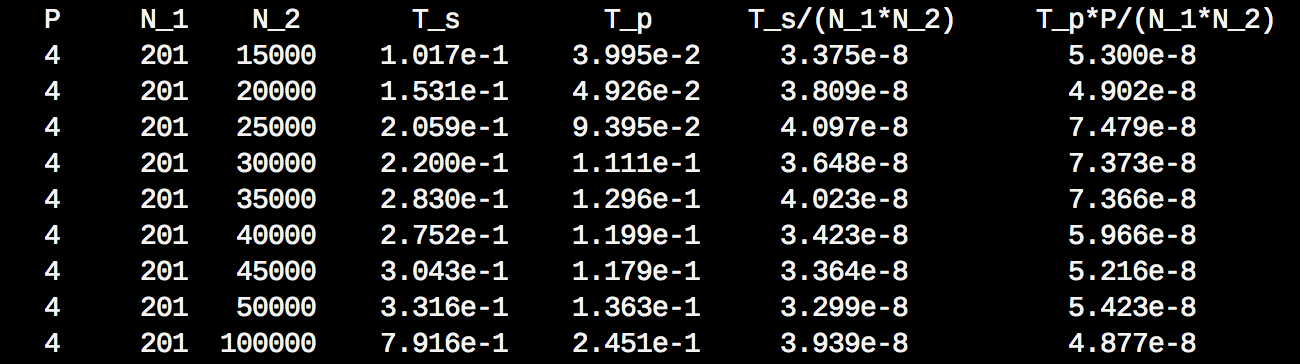
\includegraphics[width=1\textwidth]{Timing}
  \caption{Timing tables for parts b and d, $T_{s,p}$ is the timing for the sequential and parallel algorithms, respectively.}
  \label{fig:timing}
\end{figure}

See Figure~\ref{fig:timing} for timings. The order of the algorithm is $\mathcal{O}(N_1N_2)$, this is reflected in the table.

% \begin{table}
% \centering
% \begin{tabular}{|cc|ccc|}
% \hline
% \hline\\[-0.35cm]
%   $N_1$ & $N_2$ &  time& time/$(N_1+N_2)$& SD \\[0.05cm]
% \hline
% \hline
%  200 & 1000 & 7.16e-03 & 5.97e-06 & 0.000852754\\
%  200 & 10000 & 6.09e-02 & 5.97e-06 & 0.00201876\\
%  200 & 100000 & 6.66e-01 & 6.65e-06 & 0.0187756\\
%  200 & 1000000 & 6.59e+00 & 6.58e-06 & 0.217125\\
% \hline
% \hline
% \end{tabular}
% \caption{Timing table for question 4.}
% \label{tab:results}
% \end{table}


\subsection*{c}

See functions {\tt best\_match\_leaf, best\_match\_combine, best\_match\_root } and {\tt best\_match\_par}

\subsection*{d}
See Figure~\ref{fig:timing} for timings. For large enough $N_1$, $N_2$ ($\approx (100,1000)$) it seems that the parallel sequence match algorithm is better. However, when $N_1>N_2$ then the sequential version of the algorithm is preferable.


\end{document}




